\section{Measuring Possible Surveillance Opportunities}
\label{measure}
As Internet traffic crosses international borders, it becomes subject to the wiretapping policies of the national jurisdiction in which it is transitting.  Some countries, such as the United States, are well known for wiretapping policies.  We take Brazil as a case study in measuring where Brazilian Internet users' traffic is going and how often; this shows how much possible surveillance could currently be conducted on Brazilians' traffic.  The methods we use are general and can be applied to other countries of interest.

\subsection{Procedure}
Our methods for measuring where traffic paths go use the data-plane; we analyze the reported hops of traceroute measurements to find which countries are on the path from a Brazilian client to a popular domain.  For this study, we used RIPE Atlas probes in Brazil, specifically the set of probes that had unique ASes in the country (22 probes).  The destinations for traceroutes are the Brazilian Alexa Top 100 domains, as well as the third party domains within the response bodies of the 100 domains.  There are three main steps to our measurement procedure: traceroute generation and collection, transformation of traceroutes to country-level paths, and path analysis.

{\bf Step 1.} The first step is to curl each of the Brazilian Alexa Top 100 domains, and extract the third party domains from the response body.  These third party domains will each be fetched by the client when the original webpage is rendered in the browser.  Next, the 22 RIPE Atlas probes in Brazil will locally resolve each domain (and third party domain) by running a DNS measurement.  The local resolution is representative of a DNS response that an Internet user in Brazil would receive.  Once the DNS responses are received for all DNS measurements, the IP addresses are consolidated into a list of /24 subnets that cover the set of IP addresses; this is done because all IP addresses in a /24 network should geolocate to the same country.  The last part of this step is running traceroutes from the 22 RIPE Atlas probes to a single IP address in each of the /24 subnets calculated from the DNS responses.  The measurements were run using paris traceroute and each (probe, destination IP) pair was used twice: once using ICMP traceroute and once using TCP traceroute.  

{\bf Step 2.}  Step 2 generates country-level paths from the set of traceroutes produced during Step 1.  Using MaxMind \annie{or Digital Envoy}, each IP address was geolocated at a country granularity.  This resulted in a set of country-level paths.  \annie{possibly mention any differences between MaxMind and Digital Envoy?}

{\bf Step 3.}  After calculating country-level paths, we perform different data analysis to find where traffic travels.  We look for countries that are on the path between the client and teh destination, but are not the destination's country.  These countries can still conduct surveillance on the traffic, but there's also the possibility that a different path to the destination can avoid the given country.  A different analysis can show the countries in which the path ends, this is where the content is hosted.  It's important to note that the destinations found in this study could change if the content is georeplicated in other countries.  On the otherhand, if it is not georeplicated, then the destination's country is unavoidable.  Lastly, we look at how much tromboning occurs - a tromboning path is one that starts and ends in Brazil, but also traverses at least one other country.  These paths are interesting because they should not be exiting the country if the destination is in the country of origin.  

\subsection{Results}
Here we discuss our findings on which countries transit Brazilian web traffic, which countries host popular content for Brazilians, and to which countries Brazilian traffic trombones.  

\begin{figure*}
\centering
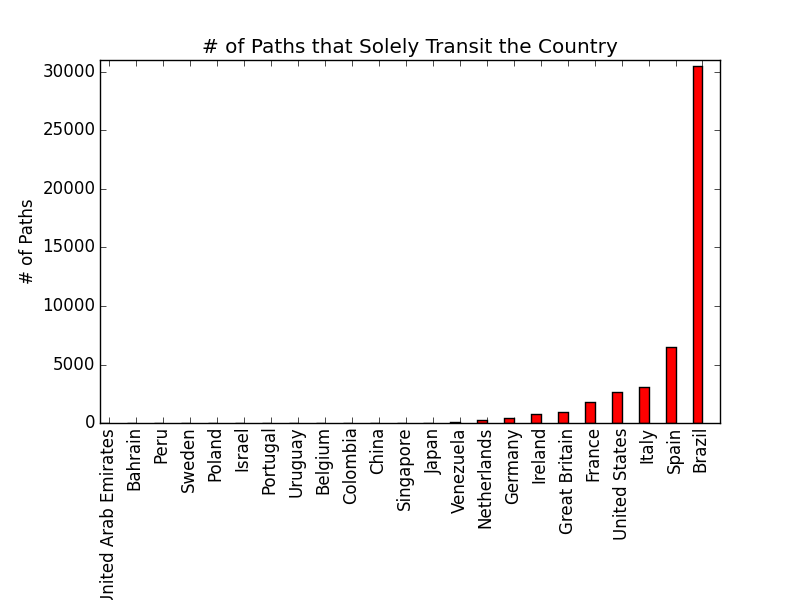
\includegraphics[width=.8\textwidth]{transit_graph_no_zero}
\caption{The number of paths that solely transit a country (do not end in the country).}
\label{fig:transit}
\end{figure*}

Figure \ref{fig:transit} shows the number of paths that transit different countries.  Note that these numbers are calculated for when the country is \textit{only} on the path and \textit{not the destination country}.  We can see that Brazil is most commonly on the path, which is expected because all paths originate from Brazil.  A few countries see a significant amount of traffic; Spain transits 17.6\% of the paths, Italy transits 8.4\% of the paths, and the United States transits 7.3\% of the paths.  Any country that is on the path has the ability to conduct surveillance on Brazilian traffic.  

More revealing than the transit-only countries, the paths that end in countries other than Brazil show that web content for Brazilian Internet users is not primarily hosted in Brazil.  The number of paths that end in different countries are shown in Figure \ref{fig:host}.  The country that hosts the most significant amount of web content is the United States; it was the destination country for 77\% of paths from Brazil.  If most of these domains are only hosted in the United States, then it's impossible for Brazilian clients to avoid the United States.  If the web content is georeplicated in another region, such as Europe, then Brazilian clients may be able to avoid the United States for a significant amout of their Internet traffic.  It is also worth noting that only 17\% of the paths end in Brazil, and the next most popular destination country is Ireland with 1.7\% of paths ending there.  

Tromboning paths show that local traffic isn't staying local; ideally, if a path starts and ends in the same country, then it shouldn't cross international borders.  We found that tromboning occurs for Brazilian traffic to 9 different countries.  These results can be seen in Figure \ref{fig:trombone}.  While we measured 4.2\% of all paths trombone, 81\% of all tromboning paths go through the United States.  For 4.2\% of the traffic, foreign countries can conduct surveillance because the traffic is not staying local (but should be). 

\begin{figure*}[t!]
\centering
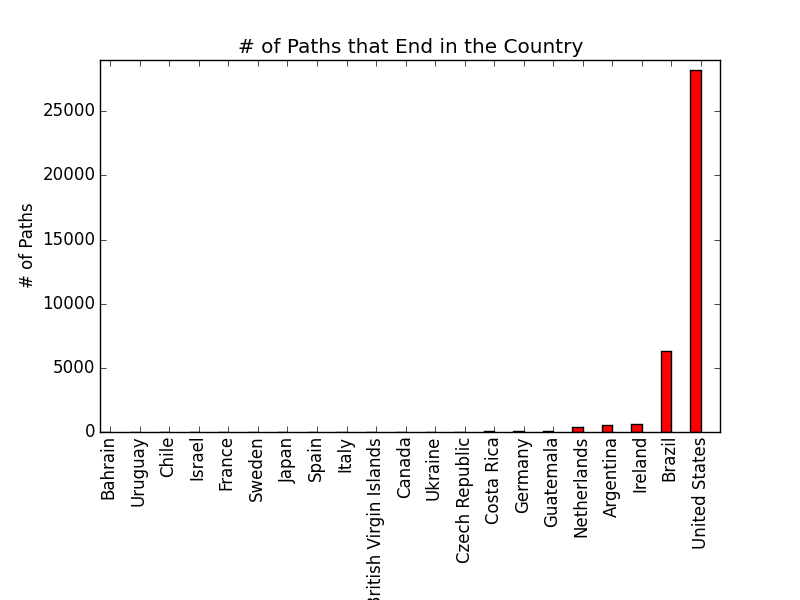
\includegraphics[width=.8\textwidth]{host_graph_no_zero}
\caption{The number of paths that end in a country.}
\label{fig:host}
\end{figure*} 

\begin{figure}
\centering
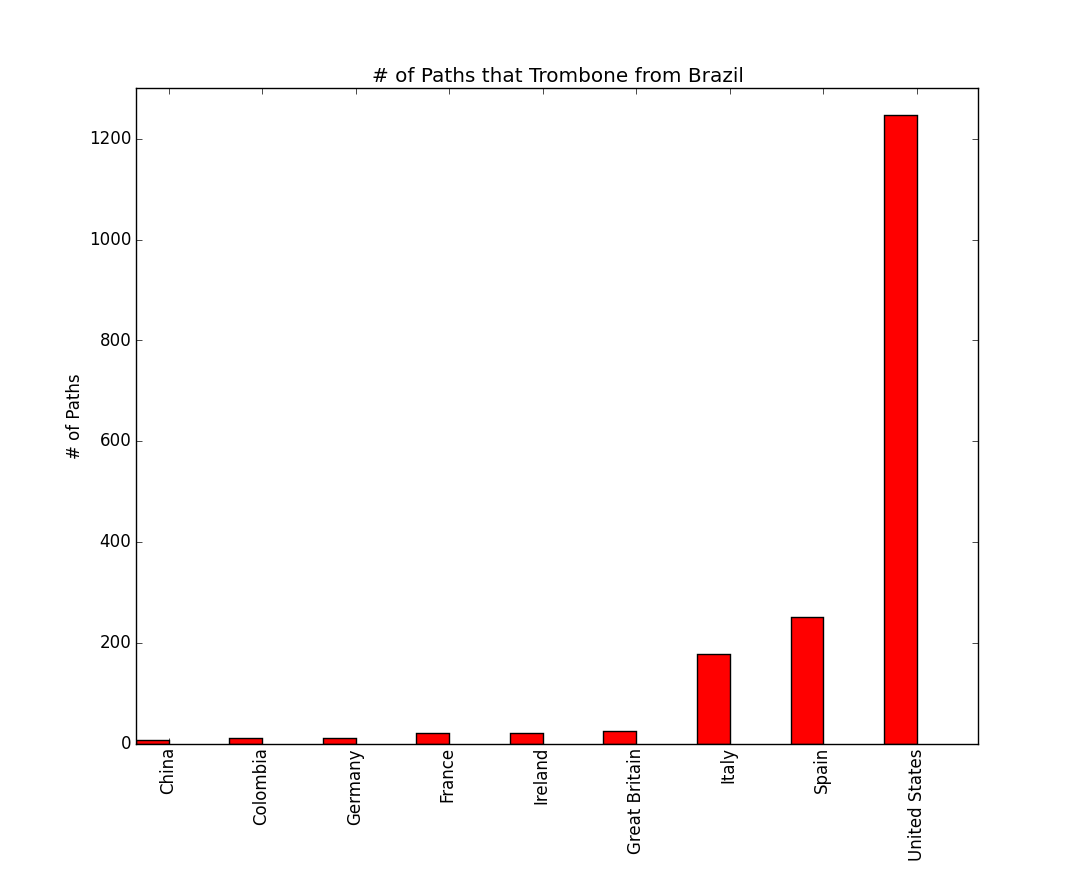
\includegraphics[width=.5\textwidth]{trombone_graph}
\caption{The number of paths that start and end in Brazil, but pass through another country.}
\label{fig:trombone}
\end{figure}

These results show that there are numerous opportunities for foreign countries to conduct surveillance on Brazilian citizens because of interdomain routing.  This motivates our system, \system{}, which allows clients anywhere in the world to reduce the number of opportunities that their traffic can be wiretapped by avoiding any country of interest.  
